\section{Chasis y cubierta del módulo exterior}
\label{app:diseno-exterior}

\subsection{Lista de materiales}

\vfill

\begin{table}[H]
\caption{Lista de materiales del módulo exterior}
\label{tab:example}
\begin{tabularx}{\textwidth}{cX}
\toprule
\headingc{Cantidad} & \headingc{Descripción} \\
\topruleb
 1 & Hoja de metacrilato de 3mm de grosor (105mm x 70mm)\\*\midrule
 1 & Hoja de metacrilato de 2mm de grosor (125mm x 115mm)\\*\midrule
 1 & Hoja de metacrilato de 2mm de grosor (170mm x 160mm)\\*\midrule
 4 & Tuercas de nylon M3 nylon\\*\midrule
 2 & Tornillos de nylos con cabeza Phillips M3 x 6mm\\*\midrule
 4 & Tornillo de nylon con tuerca integrada M3 x 6mm + 10mm\\*\midrule
 1 & Imán neodimio avellanado ($\diameter$30mm)\\*\midrule
 1 & Tornillo avellanado M3 x 10mm\\*\midrule
 2 & Tuercas de acero M3\\*\midrule
-- & Arandela(s)\\*\bottomrule
\end{tabularx}
\end{table}

\vfill

\subsection{Boceto del chasis del módulo exterior}

\vfill

\begin{figure}[H]
  \centering
  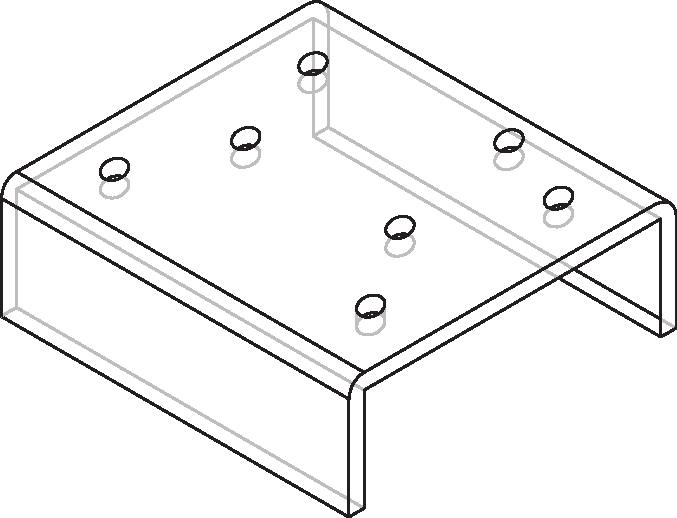
\includegraphics[width=0.6\columnwidth]{../design/exterior-skeleton-design}
  \caption{Boceto del chasis del módulo exterior}
  \label{fig:exterior-skeleton-design}
\end{figure}

\vfill

\subsection{Mecanizado del chasis del módulo exterior}

\vfill

\begin{figure}[H]
  \centering
  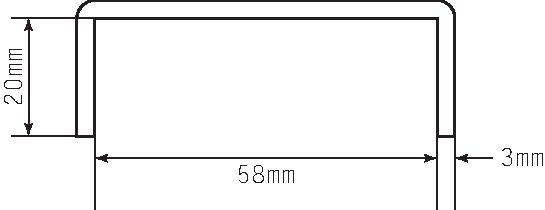
\includegraphics[width=0.8\columnwidth]{../design/exterior-skeleton-side}
  \caption{Doblado del chasis (vista lateral)}
  \label{fig:exterior-skeleton-side}
\end{figure}

\vfill

\clearpage

\begin{figure}
  \centering
  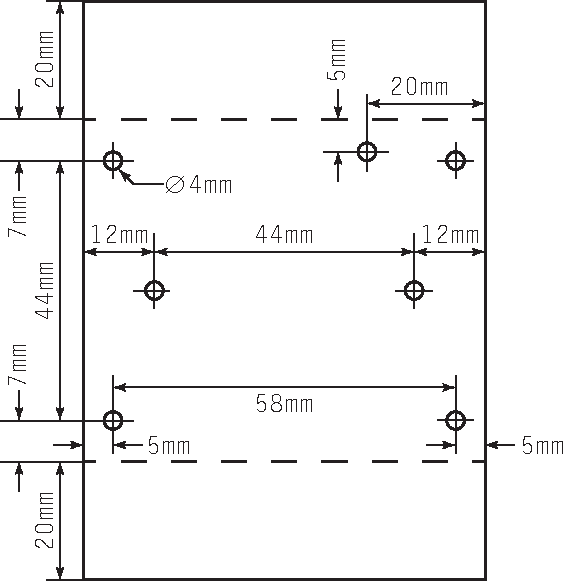
\includegraphics[height=0.8\columnwidth]{../design/exterior-skeleton-blueprint}
  \caption{Diseño del corte del chasis del módulo exterior}
  \label{fig:skeleton-skeleton-blueprint}
\end{figure}

\clearpage

\subsection{Boceto de la cubierta del módulo exterior}

\vfill

\begin{figure}[H]
  \centering
  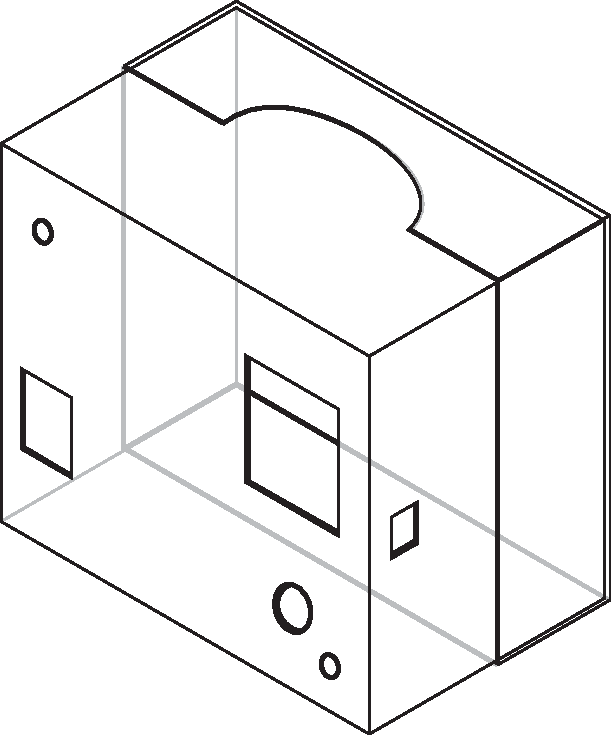
\includegraphics[width=0.6\columnwidth]{../design/exterior-body-design}
  \caption{Boceto de la cubierta del módulo exterior}
  \label{fig:exterior-body-design}
\end{figure}

\vfill

\subsection{Mecanizado de la cubierta del módulo exterior}

\vfill

\begin{figure}[H]
  \centering
  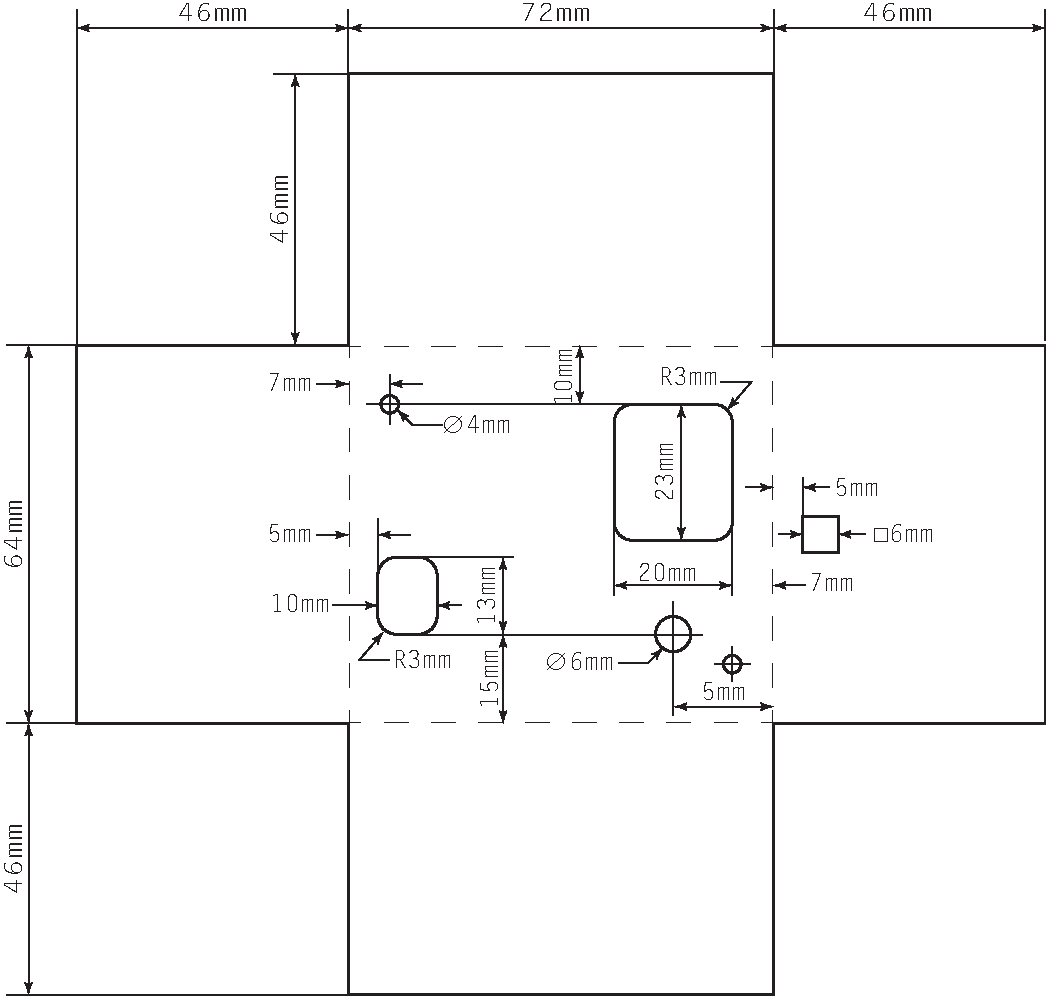
\includegraphics[width=1\columnwidth]{../design/exterior-body-blueprint}
  \caption{Diseño del corte de la cubierta del módulo exterior (cuerpo principal)}
  \label{fig:exterior-body-blueprint}
\end{figure}

\vfill

\clearpage

\begin{figure}
  \centering
  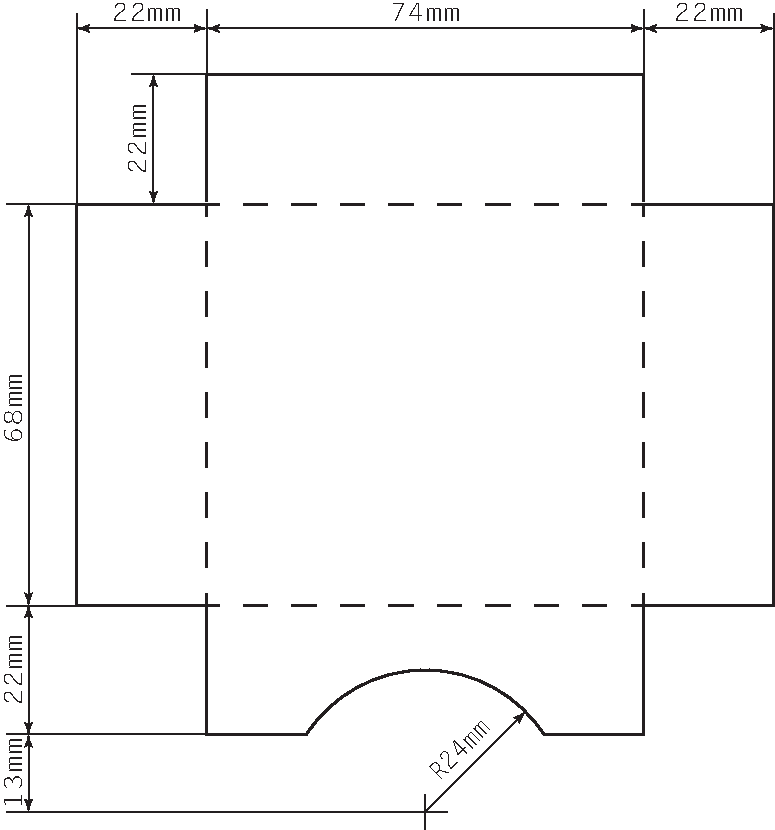
\includegraphics[height=1\columnwidth]{../design/exterior-cover-blueprint}
  \caption{Diseño del corte de la cubierta del módulo exterior (tapa)}
  \label{fig:exterior-cover-blueprint}
\end{figure}



